\documentclass[12pt,a4paper]{article}
\usepackage[polish]{babel}
\usepackage[T1]{fontenc}
\usepackage[utf8x]{inputenc}
\usepackage{hyperref}
\usepackage{url}
\usepackage{graphicx}

\addtolength{\hoffset}{-1.5cm}
\addtolength{\marginparwidth}{-1.5cm}
\addtolength{\textwidth}{3cm}
\addtolength{\voffset}{-1cm}
\addtolength{\textheight}{2.5cm}
\setlength{\topmargin}{0cm}
\setlength{\headheight}{0cm}

\newcommand{\si}{ś}
\begin{document}
	
	\title{Dokumentacja projektu\\ Gry w UNITY i C\#}
	\author{Kamil Kryus, grupa poniedziałkowa}
	\date{\today}
	
	\maketitle
	\newpage
	\section*{Część I}
	\subsection*{Opis programu}
	W ramach przedmiotu został stworzony program według następującego polecenia (umieszczonego na platformie polsl): \\
	Projekt należy zaproponować na laboratorium, a następnie wrzucić na platformę wersję do oceny (pełna solucja, wersja skompilowana, dokumentacja). Ocena będzie wystawiona w trakcie lab w styczniu.

Gra 3D powinna zawierać:

a) menu

b) linię fabularną

c) obsługę ruchu myszy/klawiatury

d) efekty dźwiękowe

e) muzykę

f) przeciwny itd.
	\subsubsection*{Linia fabularna}
	Budzimy się w \si rodku pewnego pomieszczenia posiadając broń w ręku. Rozglądając się jeste\si my w stanie dostrzec plakaty, które budzą w nas niepokój. \\
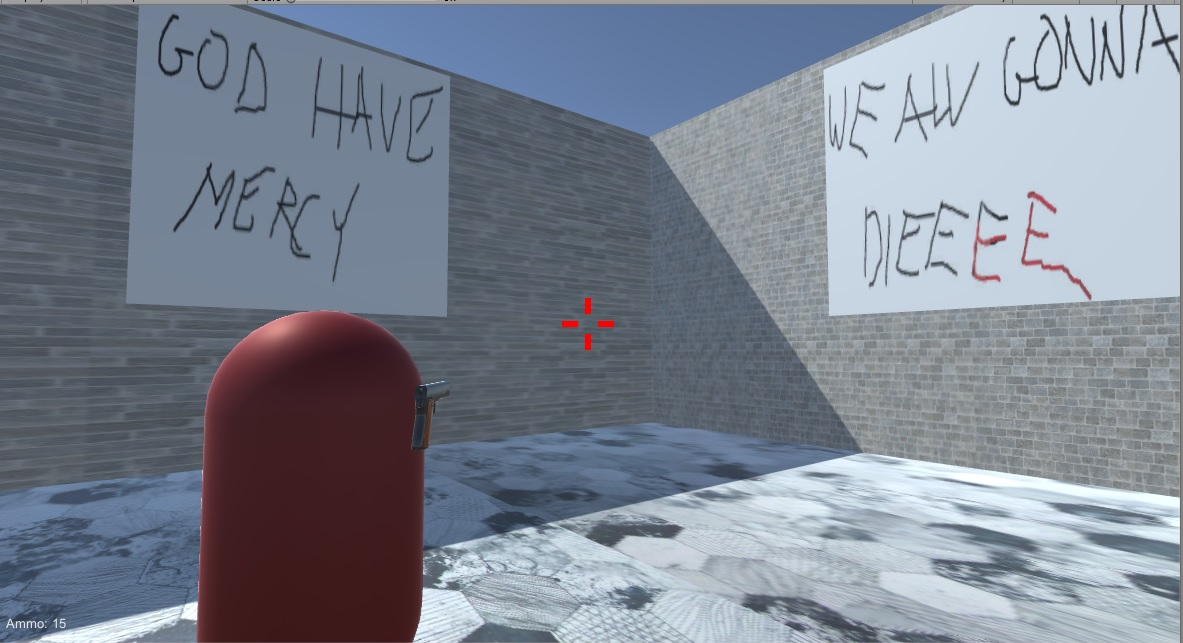
\includegraphics[height=5cm, width=5cm]{1.jpg}\\
Zastanawiając się jak możemy uciec stąd, zauważamy plakaty informujące nas o sposobie ucieczki. \\
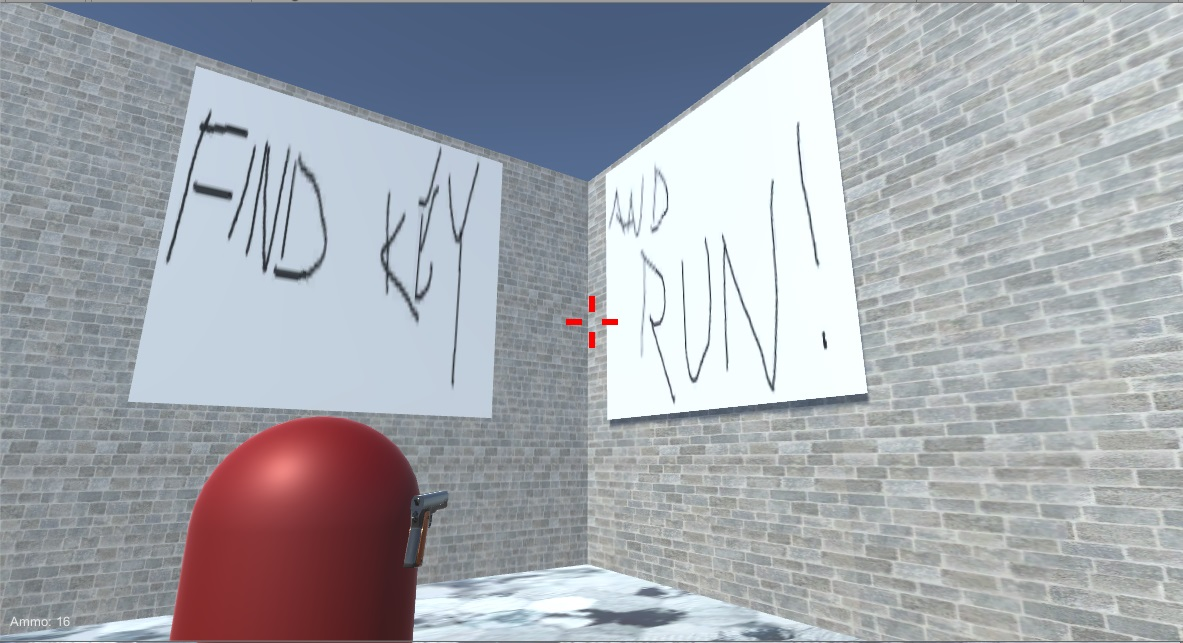
\includegraphics[height=5cm, width=5cm]{2.jpg}\\
Wychodzimy więc przez pobliską bramę i modlimy się, by zauważony stwór nas nie zauważył. Przechodząc z pokoju do pokoju i zabijając utrudniające nam ucieczkę zombie, natrafiamy w końcu na pokój, w którym znajduje się klucz.  \\
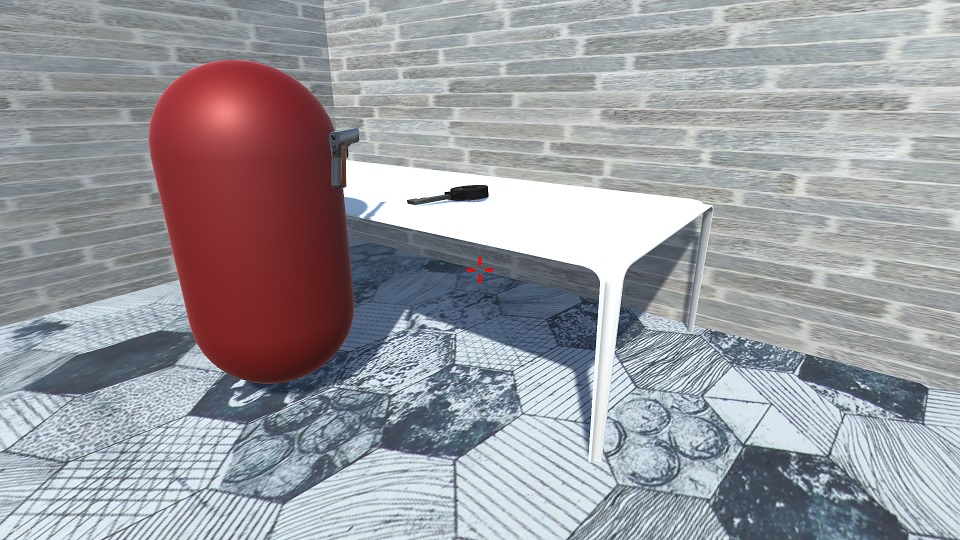
\includegraphics[height=5cm, width=5cm]{3.jpg}\\
Zabieramy go ze sobą i idziemy dalej. Docieramy aż do bramy, którą można otworzyć za pomocą tego klucza. Po wyj\si ciu na zewnątrz okazuje się, że otacza nas pustka... po czym się budzimy.


	\subsection*{Instrukcja obsługi}
	Grę włączamy poprzez dwukrotne przyci\si nięcie lewym przyciskiem myszy na ikonce gry:\\
	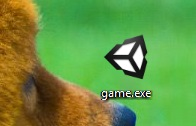
\includegraphics[height=5cm, width=5cm]{4.jpg}\\
	Po ustawieniu ustawień graficznych gry, przyciskamy przycisk Play! \\
	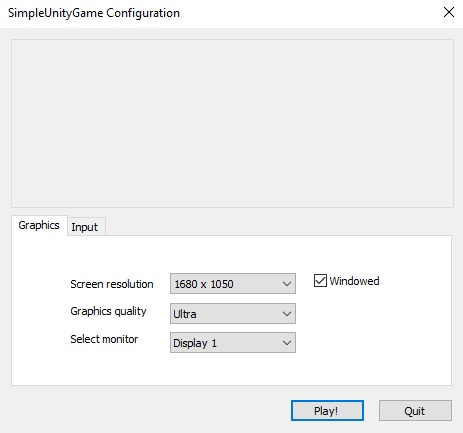
\includegraphics[height=5cm, width=5cm]{4i5.jpg}\\
	Po załadowaniu gry, aby rozpocząć grę, należy nacisnąć lewym przyciskiem myszy na przycisku Start: \\
	
\includegraphics[height=5cm, width=5cm]{5.jpg}\\
	
	Od tej chwili możemy grać. W każdej chwili jeste\si my w stanie zakończyć grę poprzez wci\si nięcie odpowiedniego przycisku (opisanego w sekcji Sterowanie).
	\subsection*{Sterowanie}
	Oto lista przycisków oraz opis ich działania: 
	\begin{itemize}
		\item[--] Esc - wyj\si cie z gry,
		\item[--]  Lewy Przycisk Myszy/Ctrl - strzał
		\item[--]  w - ruch do przodu
		\item[--]  s - ruch do tyłu
		\item[--]  a - ruch w lewo
		\item[--]  d - ruch w prawo
		\item[--] spacja - skok
		\item[--]  e - wykonanie akcji (np. otwarcie bramy, wzięcie klucza).
	\end{itemize}
	Ponadto w grze jeste\si my w stanie rozglądać się za pomocą ruchu myszy.
	\subsection*{Solucja do przejścia gry}
 	Najprostszą drogę prowadzącą od początkowej pozycji gracza do wyj\si cia przedstawia następujący obrazek wraz z legendą: \\
 	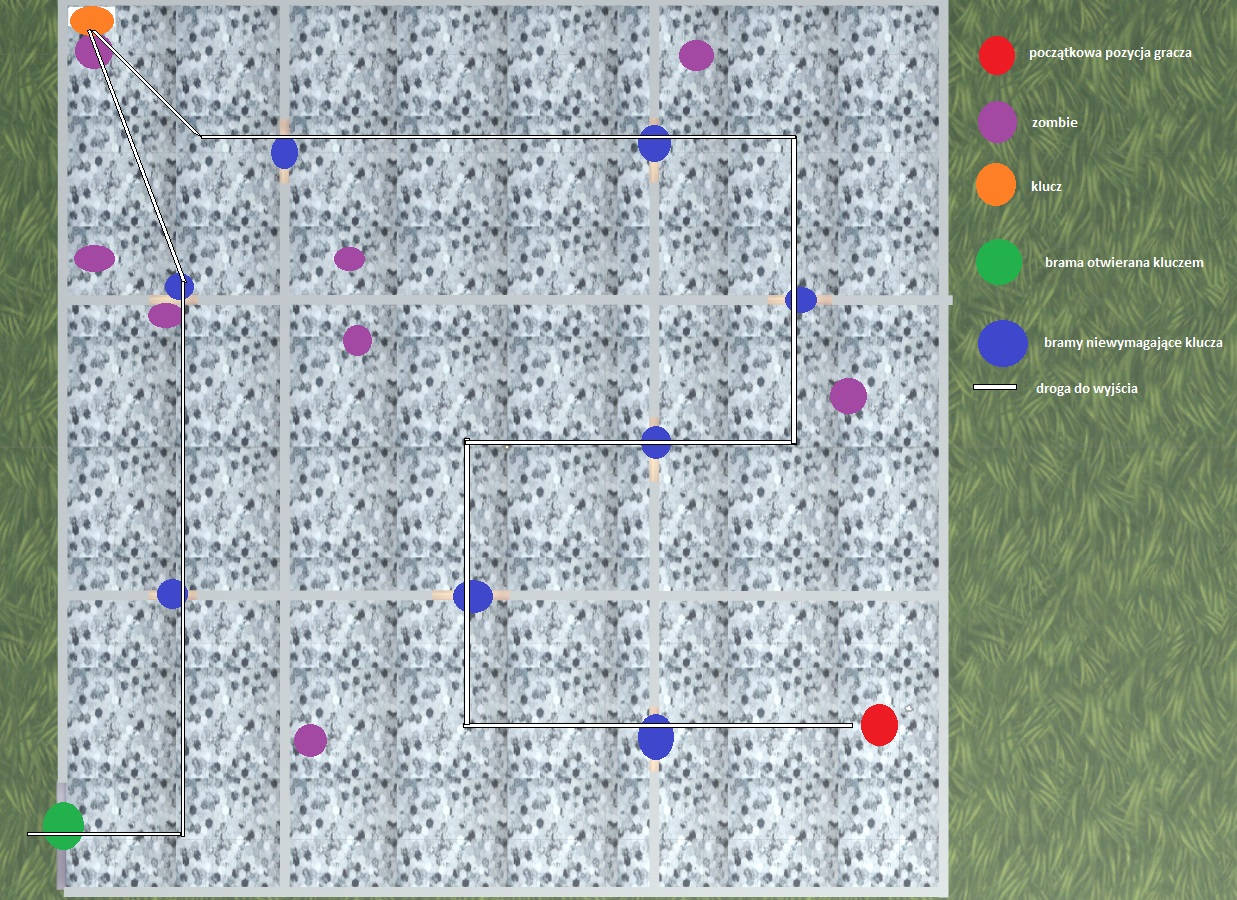
\includegraphics[height=13cm, width=15cm]{6.jpg}\\
 	Po drodze należy zabijać (lub uciekać) przeciwników za pomocą broni i otwierać bramy klawiszem akcji. Ostatnią bramę otworzymy (na obrazku zaznaczona kolorem zielonym) tylko posiadając przy sobie klucz, ktory możemy zdobyć (przyciskiem akcji) w trakcie eksploracji (pomarańczowy kolor): \\
 	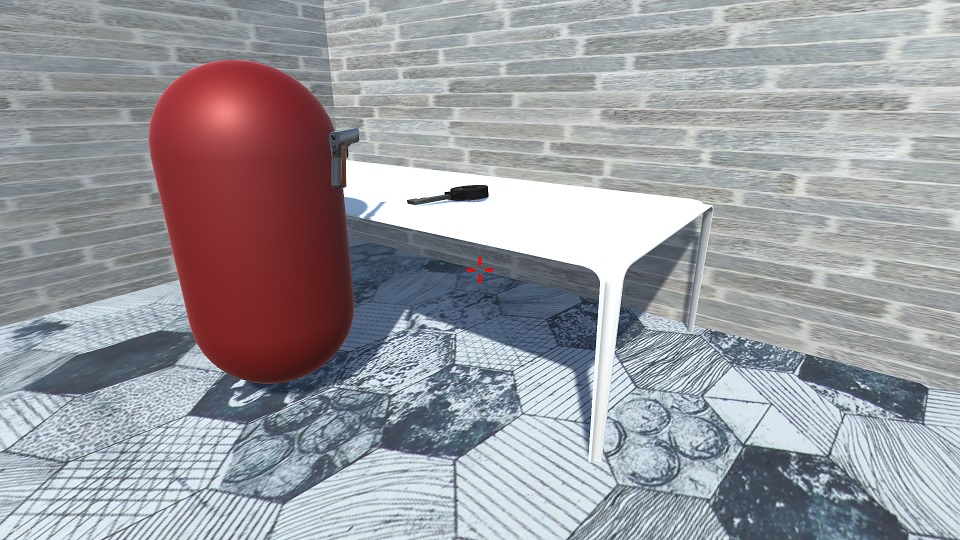
\includegraphics[height=5cm, width=5cm]{3.jpg}\\
 	Aby ukończyć grę, należy wyj\si ć z budynku, a następnie odczekać 4 sekundy.
\newpage
	\section*{Część II}
	\subsection*{Część techniczna}
	\subsubsection*{Otwieranie bram}
	Do każdej bramy podpięty jest skrypt, który wykrywa sytuację, iż obiekt gracza znalazł się blisko i wcisnął przycisk akcji. Gdy zostaną spełnione te warunki, rozpoczyna się proces w pętli obniżania pozycji bramy w osi Y, aż osiągnie pewien punkt, w którym nie jest już widoczna dla gracza. \\
	\subsubsection*{Otwieranie bramy za pomocą klucza}
	Skrypt ten działa w bardzo podobny sposób do zwykłego otwierania bramy. Mechanizm ten dodatkowo sprawdza czy klucz został zebrany przez gracza - jeżeli gracz nie wykonał tej akcji, brama nie obniży się.
	
	\subsubsection*{Zebranie klucza} 
	Ten mechanizm również działa w bardzo podobny sposób do otwierania się bram. Gdy obiekt klucza wykryje blisko\si ć gracza i wci\si nięcie klawisza akcji, modyfikuje zmienną odpowiedzialną za stan zebrania klucza i usuwa się, dzięki czemu nie widać klucza w grze po jego zebraniu.
	
	\subsubsection*{Strzelanie i ranienie przeciwników} 
	Wci\si nięcie odpowiedniego przycisku powoduje szereg animacji symulujących strzał z pistoletu. Ranienie przeciwników działa na zasadzie raycastingu - przeprowadzana jest prosta pomiędzy \si rodkiem celownika, a napotkanym obiektem. Jeżeli napotkanym obiektem jest nasz przeciwnik, to system wywołuje podpiętą metodę informując tym samym komponent o zranieniu go. Jeżeli poziom życia przeciwnika osiągnie zero, funkcje związane z poruszaniem się, atakowaniem bohatera itp. ustają.
	\subsubsection*{Zachowanie przeciwników} 
	Projekt posiada prostą sztuczną inteligencję przeciwników. Jeżeli gracz znajdzie się w pewnej odległo\si ci od przeciwnika, to ten zaczyna poruszać się i obracać w stronę gracza. Przeciwnik może również zacząć \si cigać gracza w przypadku otrzymania obrażeń. Przeciwnik jednak musi posiadać przynajmniej 1 punkt życia, aby te funkcje działały. 
	\subsubsection*{Animacje przeciwników} 
	Animacjami przeciwników zarządza kontroler, który w zależno\si ci od parametrów, wykonuje konkretną animację. Parametry natomiast są zmieniane za pomocą skryptów w zależno\si ci od wystąpienia pewnych zdarzeń.
	\subsection*{Opis działania} 
	\subsubsection*{Ściganie gracza} 
	Klasa Vector3 posiada metodę pozwalającą nam obliczyć odległo\si ć pomiędzy obiektami nazwaną Distance(). Jeżeli dystans ten jest większy niż 1.72 jednostki i jednocze\si nie mniejszy niż 30 jednostek, przeciwnik zaczyna \si cigać gracza. Jeżeli przeciwnik jest bliżej niż 2 jednostki od gracza, rozpoczyna atakować bohatera odejmując mu 1 punkt życia na klatkę, zmieniana jest również wtedy animacja. 
	\subsubsection*{Otwieranie bram} 
	Jeżeli dystans (obliczany za pomocą metody Distance() z klasy Vector3) pomiędzy graczem, a bramą jest mniejszy niż 5 jednostek, brama rozpoczyna proces otwierania się. W każdej klatce pozycja bramy na osi Y jest zmniejszana przez iloczyn czasu (w sekundach) od ostatniej klatki i własnej liczby (równej 2.5) manipulującej szybko\si cią animacji. Jeżeli pozycja bramy na osi Y osiągnie pewną liczbę, która jest wystarczająca, aby nie była widoczna dla gracza, proces się kończy.
	\subsubsection*{Obliczanie obrażeń} 
	Zarówno przeciwnik, jak i gracz zadają obrażenia o warto\si ci 1. Każdy przeciwnik ma 10 punktów życia (a tym samym potrzeba 10 strzałów by zabić go), natomiast gracz posiada aż 100 punktów życia. Jednak przeciwnicy atakują co klatkę i w przypadku ataku, gracz może bardzo szybko zginąć.
	
	
	\subsection*{Implementacja}
	\subsubsection*{Sztuczna inteligencja} 
	Zachowanie (sprawdzane w każdej klatce) przeciwników zostało zaimplementowane w następujący sposób:
	\begin{verbatim}
	if ((Vector3.Distance(playerTrans.position, this.transform.position) < 30f &&
	 life > 0) || (life < 20 && life > 0) &&
	  Vector3.Distance(playerTrans.position, this.transform.position) > 1.72f)
        {
            float step = 2.0f * Time.deltaTime;
            Vector3 targetDir = playerTrans.position - transform.position;
            targetDir.y = 0.3f;

            Vector3 newDir = Vector3.RotateTowards(transform.forward, targetDir, step, 0.0f);

            transform.rotation = Quaternion.LookRotation(newDir);
            var tmpPos = playerTrans.position;
            tmpPos.y = 0.2f;

            this.transform.position = Vector3.MoveTowards(this.transform.position, tmpPos, step);
            transform.position = new Vector3(transform.position.x, 0.2f, transform.position.z);
        }
        if (Vector3.Distance(playerTrans.position, this.transform.position) < 2f &&
         life > 0)
        {
            thisAnim.SetBool("isAttacking", true);
            Player.life -= 1;
            if (Player.life <= 0)
            {
                SceneManager.LoadScene(2);
            }
        }
        else
        {
            thisAnim.SetBool("isAttacking", false);
        }
	\end{verbatim}
	
	\subsubsection*{Raycasting} 
	System strzelania został porany ze sklepu i jedynie przystosowany do potrzeb projektu. W momencie strzału skrypt informuje odpowiedni obiekt o wydarzeniu poprzez wywołanie metody ChangeHealth().
	\begin{verbatim}		
		Ray ray = new Ray(raycastStartSpot.position, direction);
            RaycastHit hit;

            if (Physics.Raycast(ray, out hit, range))
            {
                // Warmup heat
                float damage = power;
                if (warmup)
                {
                    damage *= heat * powerMultiplier;
                    heat = 0.0f;
                }
                // Damage
                hit.collider.gameObject.SendMessageUpwards("ChangeHealth", -damage, SendMessageOptions.DontRequireReceiver);

                if (bloodyMessEnabled)
                {
                    //call the ApplyDamage() function on the enenmy CharacterSetup script
                    if (hit.collider.gameObject.layer == LayerMask.NameToLayer("Limb"))
                    {
                        Vector3 directionShot = hit.collider.transform.position - transform.position;

                    }
                }

            }
	\end{verbatim}
	Powyższy fragment kodu wywołuje metodę powiązaną z samym przeciwnikiem. Warto\si ć dmg wynosi zawsze -1.
	\begin{verbatim}
	public void ChangeHealth(int dmg)
    {
        life += dmg;
        if (life <= 0)
        {
            thisAnim.SetBool("isDead", true);
        }
    }
	\end{verbatim}



	\newpage
		\section*{Część III}
		\subsection{Blender}
		Tworząc projekt nie korzystałem z oprogramowania Blender.
		\subsection{UNITY}
		\subsubsection*{Pobrane ze sklepu} 
		\underline{Zombie} \\		
		Pobrany asset udostępniał gotowy prefabrykat, animacje, kontroler animacji oraz skrypty. Dla potrzeb projektu, skorzystałem jedynie z niektórych animacji oraz samego modelu zombie.\\
		
		\noindent \underline{Bronie i system strzelania} \\		
		Udostępnione materiały zawierały bardzo dużo funkcjonalno\si ci, jednak do finalnego projektu zostało użyte tylko kilka. Model (jednej) broni, skrypty związane ze strzelaniem i raycastingiem oraz animacje. \\
		
		\noindent \underline{Menu} \\		
		Chociaż pobrane ze sklepu menu zapewniało pełną funkcjonalno\si ć, skorzystałem głównie pojawienia się przycisków w widocznym miejscu kamery oraz skryptów powiązanych z reakcjami na kliknięcie przycisków. \\
		
		\noindent \underline{Model klucza i stołu} \\
		Dla potrzeb projektu skorzystałem z modelu klucza i stołu. Funkcjonalno\si ć oraz inne modele nie zostały wykorzystane.
		
		\noindent \subsubsection*{Własne} 
		W czasie pracy nad projektem następujące elementy zostały stworzone przeze mnie:
		\begin{itemize}
		\item[--] Linia fabularna

		\item[--] Otwieranie bram
		\item[--] Sztuczna inteligencja przeciwników
		\item[--] Budowla

		\end{itemize}

	\section*{Pełen kod programu}
	
	\begin{itemize}
	\item BackToMenu.cs
	\begin{verbatim}
	using System.Collections;
using System.Collections.Generic;
using UnityEngine;
using UnityEngine.SceneManagement;

public class BackToMenu : MonoBehaviour {

	// Use this for initialization
	void Start () {
		
	}
	
	// Update is called once per frame
	void Update () {
        if (Input.GetKeyDown(KeyCode.Escape))
        {
            Cursor.lockState = CursorLockMode.None;
            SceneManager.LoadScene(0);
        }
    }
}

	\end{verbatim}
	\item CollectKey.cs
	\begin{verbatim}
	using System.Collections;
using System.Collections.Generic;
using UnityEngine;

public class CollectKey : MonoBehaviour {

    public GameObject key;
    private Transform playerTrans = null;
    void Start()
    {
        playerTrans = GameObject.Find("Player").transform;
    }
    void Update()
    {
        if (Input.GetKeyDown(KeyCode.E))
        {
            if (Vector3.Distance(playerTrans.position, this.transform.position) < 5f)
            {
                Player.hasKey = true;
                Destroy(key);
            }
        }
    }
}

	\end{verbatim}
	\item FinishGame.cs
	\begin{verbatim}
	using System.Collections;
using System.Collections.Generic;
using UnityEngine;
using UnityEngine.SceneManagement;
using System;

public class FinishGame : MonoBehaviour {

	// Use this for initialization
	void Start () {
		
	}
	
	// Update is called once per frame
	void Update () {
		
	}

    private void OnTriggerEnter(Collider other)
    {
        StartCoroutine(Wait(4.0f));
    }

    IEnumerator Wait(float seconds)
    {
        yield return new WaitForSeconds(seconds);
        SceneManager.LoadScene(3);
    }
}

	\end{verbatim}
	\item MouseLook.cs
	\begin{verbatim}
	using System.Collections;
using System.Collections.Generic;
using UnityEngine;

public class MouseLook : MonoBehaviour {

    // Use this for initialization
    Vector2 _mouseAbsolute;
    Vector2 _smoothMouse;

    public Vector2 clampInDegrees = new Vector2(360, 180);
    public bool lockCursor;
    public Vector2 sensitivity = new Vector2(2, 2);
    public Vector2 smoothing = new Vector2(3, 3);
    public Vector2 targetDirection;
    public Vector2 targetCharacterDirection;

    // Assign this if there's a parent object controlling motion, such as a Character Controller.
    // Yaw rotation will affect this object instead of the camera if set.
    public GameObject characterBody;

    void Start()
    {
        // Set target direction to the camera's initial orientation.
        targetDirection = transform.localRotation.eulerAngles;

        // Set target direction for the character body to its inital state.
        if (characterBody)
            targetCharacterDirection = characterBody.transform.localRotation.eulerAngles;
    }

    void Update()
    {
        // Ensure the cursor is always locked when set
        if (lockCursor)
        {
            Cursor.lockState = CursorLockMode.Locked;
        }

        // Allow the script to clamp based on a desired target value.
        var targetOrientation = Quaternion.Euler(targetDirection);
        var targetCharacterOrientation = Quaternion.Euler(targetCharacterDirection);

        // Get raw mouse input for a cleaner reading on more sensitive mice.
        var mouseDelta = new Vector2(Input.GetAxisRaw("Mouse X"), Input.GetAxisRaw("Mouse Y"));

        // Scale input against the sensitivity setting and multiply that against the smoothing value.
        mouseDelta = Vector2.Scale(mouseDelta, new Vector2(sensitivity.x * smoothing.x, sensitivity.y * smoothing.y));

        // Interpolate mouse movement over time to apply smoothing delta.
        _smoothMouse.x = Mathf.Lerp(_smoothMouse.x, mouseDelta.x, 1f / smoothing.x);
        _smoothMouse.y = Mathf.Lerp(_smoothMouse.y, mouseDelta.y, 1f / smoothing.y);

        // Find the absolute mouse movement value from point zero.
        _mouseAbsolute += _smoothMouse;

        // Clamp and apply the local x value first, so as not to be affected by world transforms.
        if (clampInDegrees.x < 360)
            _mouseAbsolute.x = Mathf.Clamp(_mouseAbsolute.x, -clampInDegrees.x * 0.5f, clampInDegrees.x * 0.5f);

        // Then clamp and apply the global y value.
        if (clampInDegrees.y < 360)
            _mouseAbsolute.y = Mathf.Clamp(_mouseAbsolute.y, -clampInDegrees.y * 0.5f, clampInDegrees.y * 0.5f);

        transform.localRotation = Quaternion.AngleAxis(-_mouseAbsolute.y, targetOrientation * Vector3.right) * targetOrientation;

        // If there's a character body that acts as a parent to the camera
        if (characterBody)
        {
            var yRotation = Quaternion.AngleAxis(_mouseAbsolute.x, Vector3.up);
            characterBody.transform.localRotation = yRotation * targetCharacterOrientation;
        }
        else
        {
            var yRotation = Quaternion.AngleAxis(_mouseAbsolute.x, transform.InverseTransformDirection(Vector3.up));
            transform.localRotation *= yRotation;
        }
    }
}

	\end{verbatim}
	\item Movement.cs
	\begin{verbatim}
	using System.Collections;
using System.Collections.Generic;
using UnityEngine;

public class Movement : MonoBehaviour {

    //Variables
    public float speed = 6.0F;
    public float jumpSpeed = 8.0F;
    public float gravity = 20.0F;
    private Vector3 moveDirection = Vector3.zero;

    void Update()
    {
        CharacterController controller = GetComponent<CharacterController>();
        // is the controller on the ground?
        if (controller.isGrounded)
        {
            //Feed moveDirection with input.
            moveDirection = new Vector3(Input.GetAxis("Horizontal"), 0, Input.GetAxis("Vertical"));
            moveDirection = transform.TransformDirection(moveDirection);
            //Multiply it by speed.
            moveDirection *= speed;
            //Jumping
            if (Input.GetButton("Jump"))
                moveDirection.y = jumpSpeed;

        }
        //Applying gravity to the controller
        moveDirection.y -= gravity * Time.deltaTime;
        //Making the character move
        controller.Move(moveDirection * Time.deltaTime);
    }
}

	\end{verbatim}
	\item OpenGate.cs
	\begin{verbatim}
	using System.Collections;
using System.Collections.Generic;
using UnityEngine;

public class OpenGate : MonoBehaviour
{
    private float animationSpeed = 2.5f;
    public GameObject player;
    private Transform playerTransform;

    public AudioSource audioSource;
    public AudioClip gateOpeningClip;

    void Start()
    {
        playerTransform = player.transform;
    }
    void Update()
    {
        if (Input.GetKeyDown(KeyCode.E))
        {
            if (Vector3.Distance(playerTransform.position, this.transform.position) < 5f)
            {
                StartCoroutine(MoveGate());
            }
        }
    }

    public IEnumerator MoveGate()
    {
        audioSource.PlayOneShot(gateOpeningClip);
        while (transform.localPosition.y > 16.35)
        {
            transform.localPosition = new Vector3(transform.localPosition.x, transform.localPosition.y - Time.deltaTime * animationSpeed, transform.localPosition.z);
            yield return null;
        }
    }
}



	\end{verbatim}
	\item OpenGateWithkey.cs
	\begin{verbatim}
	using System.Collections;
using System.Collections.Generic;
using UnityEngine;

public class OpenGateWithKey : MonoBehaviour
{
    private float animationSpeed = 2.5f;
    public GameObject player;
    private Transform playerTransform;
    public AudioSource audioSource;
    public AudioClip gateOpeningClip;

    void Start()
    {
        playerTransform = player.transform;
    }
    void Update()
    {
        if (Input.GetKeyDown(KeyCode.E))
        {
            if (Vector3.Distance(playerTransform.position, this.transform.position) < 5f && Player.hasKey)
            {
                StartCoroutine(MoveGate());
            }
        }
    }

    public IEnumerator MoveGate()
    {
        audioSource.PlayOneShot(gateOpeningClip);
        while (transform.localPosition.y > -7.37)
        {
            transform.localPosition = new Vector3(transform.localPosition.x, transform.localPosition.y - Time.deltaTime * animationSpeed, transform.localPosition.z);
            yield return null;
        }
    }
}

	\end{verbatim}
	\item Player.cs
	\begin{verbatim}
	using System.Collections;
using System.Collections.Generic;
using UnityEngine;
using UnityEngine.SceneManagement;

public class Player : MonoBehaviour {

    public static bool hasKey;
    public static int life = 100;

	// Use this for initialization
	void Start () {
		
	}
	
	// Update is called once per frame
	void Update () {
        
    }
}

	\end{verbatim}
	\item ZombieBehaviour.cs
	\begin{verbatim}
	using System.Collections;
using System.Collections.Generic;
using UnityEngine;
using UnityEngine.SceneManagement;

public class ZombieBehaviour : MonoBehaviour
{
    public int life = 10;
    private Animator thisAnim;

    private Transform playerTrans = null;
    void Start()
    {
        playerTrans = GameObject.Find("Player").transform;
        thisAnim = GetComponent<Animator>();
    }
    void Update()
    {
        if ((Vector3.Distance(playerTrans.position, this.transform.position) < 30f && life > 0) || (life < 20 && life > 0) && Vector3.Distance(playerTrans.position, this.transform.position) > 1.72f)
        {
            float step = 2.0f * Time.deltaTime;
            Vector3 targetDir = playerTrans.position - transform.position;
            targetDir.y = 0.3f;

            Vector3 newDir = Vector3.RotateTowards(transform.forward, targetDir, step, 0.0f);

            transform.rotation = Quaternion.LookRotation(newDir);
            var tmpPos = playerTrans.position;
            tmpPos.y = 0.2f;

            this.transform.position = Vector3.MoveTowards(this.transform.position, tmpPos, step);
            transform.position = new Vector3(transform.position.x, 0.2f, transform.position.z);
        }
        if (Vector3.Distance(playerTrans.position, this.transform.position) < 2f && life > 0)
        {
            thisAnim.SetBool("isAttacking", true);
            Player.life -= 1;
            if (Player.life <= 0)
            {
                SceneManager.LoadScene(2);
            }
        }
        else
        {
            thisAnim.SetBool("isAttacking", false);
        }
    }

    public void ChangeHealth(int dmg)
    {
        life += dmg;
        if (life <= 0)
        {
            thisAnim.SetBool("isDead", true);
        }
    }
}

	\end{verbatim}
	\end{itemize}
\end{document}
